\documentclass{article}

\usepackage{tikz-feynman}

\begin{document}

\begin{tikzpicture}
	\begin{feynman}
		\vertex (a) {\(u\)};
		\vertex [right=of a](b);
		\vertex [above right=of b](c){\(d\)};
		\vertex [below=of b] (d);
		\vertex [below=of d] (e);
		\vertex [below=of e] (f);
		\vertex [left=of f] (g) {\(u\)};
		\vertex [below right=of f] (h) {\(d\)};
		\vertex [right=of d] (i);
		\vertex [above right=of i] (l){\(\bar{\tau}\)};
		\vertex [right=of i] (m){\(\nu_{\tau}\)};
		\vertex [right=of e] (o);
		\vertex [right=of o] (p){\(\bar{\tau}\)};
		\vertex [below right=of o] (q){\(\nu_{\tau}\)};
		
		
		\diagram* {
			(a) -- [fermion] (b) -- [fermion] (c),
			(b) -- [scalar, edge label'=\(W^{+}\)] (d) -- [scalar, edge label'=\(Z^{0} ||  \gamma\)] (e) -- [scalar, edge label'=\(W^{+}\)] (f);
			(g) -- [fermion] (f) -- [fermion] (h);
			(d) -- [scalar, edge label'=\(W^{+}\)] (i);
			(l) -- [fermion] (i) -- [fermion] (m);
			(e) -- [scalar, edge label'=\(W^{+}\)] (o);
			(p) -- [fermion] (o) -- [fermion] (q);
		};
	\end{feynman}
\end{tikzpicture}

\begin{tikzpicture}
	\begin{feynman}
		\vertex (a) {\(d\)};
		\vertex [right=of a](b);
		\vertex [above right=of b](c){\(u\)};
		\vertex [below=of b] (d);
		\vertex [below=of d] (e);
		\vertex [below=of e] (f);
		\vertex [left=of f] (g) {\(d\)};
		\vertex [below right=of f] (h) {\(u\)};
		\vertex [right=of d] (i);
		\vertex [above right=of i] (l){\(\tau\)};
		\vertex [right=of i] (m){\(\bar{\nu_{\tau}}\)};
		\vertex [right=of e] (o);
		\vertex [right=of o] (p){\(\tau\)};
		\vertex [below right=of o] (q){\(\bar{\nu_{\tau}}\)};
		
		
		\diagram* {
			(a) -- [fermion] (b) -- [fermion] (c),
			(b) -- [scalar, edge label'=\(W^{-}\)] (d) -- [scalar, edge label'=\(Z^{0} ||  \gamma\)] (e) -- [scalar, edge label'=\(W^{-}\)] (f);
			(g) -- [fermion] (f) -- [fermion] (h);
			(d) -- [scalar, edge label'=\(W^{-}\)] (i);
			(m) -- [fermion] (i) -- [fermion] (l);
			(e) -- [scalar, edge label'=\(W^{-}\)] (o);
			(q) -- [fermion] (o) -- [fermion] (p);
		};
	\end{feynman}
\end{tikzpicture}

\begin{tikzpicture}
	\begin{feynman}
		\vertex (a) {\(u\)};
		\vertex [right=of a](b);
		\vertex [above right=of b](c){\(u\)};
		\vertex [below=of b] (d);
		\vertex [below=of d] (e);
		\vertex [below=of e] (f);
		\vertex [left=of f] (g) {\(u\)};
		\vertex [below right=of f] (h) {\(d\)};
		\vertex [right=of d] (i);
		\vertex [above right=of i] (l){\(\tau\)};
		\vertex [right=of i] (m){\(\bar{\tau}\)};
		\vertex [right=of e] (o);
		\vertex [right=of o] (p){\(\bar{\tau}\)};
		\vertex [below right=of o] (q){\(\nu_{\tau}\)};
		
		
		\diagram* {
			(a) -- [fermion] (b) -- [fermion] (c),
			(b) -- [scalar, edge label'=\(Z^{0}\)] (d) -- [scalar, edge label'=\(Z^{0}\)] (e) -- [scalar, edge label'=\(W^{+}\)] (f);
			(h) -- [fermion] (f) -- [fermion] (g);
			(d) -- [scalar, edge label'=\(Z^{0}\)] (i);
			(m) -- [fermion] (i) -- [fermion] (l);
			(e) -- [scalar, edge label'=\(W^{+}\)] (o);
			(p) -- [fermion] (o) -- [fermion] (q);
		};
	\end{feynman}
\end{tikzpicture}

\begin{tikzpicture}
	\begin{feynman}
		\vertex (a) {\(u\)};
		\vertex [right=of a](b);
		\vertex [above right=of b](c){\(u\)};
		\vertex [below=of b] (d);
		\vertex [below=of d] (e);
		\vertex [below=of e] (f);
		\vertex [left=of f] (g) {\(u\)};
		\vertex [below right=of f] (h) {\(d\)};
		\vertex [right=of d] (i);
		\vertex [above right=of i] (l){\(\tau\)};
		\vertex [right=of i] (m){\(\bar{\tau}\)};
		\vertex [right=of e] (o);
		\vertex [right=of o] (p){\(\tau\)};
		\vertex [below right=of o] (q){\(\bar{\nu_{\tau}}\)};
		
		
		\diagram* {
			(a) -- [fermion] (b) -- [fermion] (c),
			(b) -- [scalar, edge label'=\(Z^{0}\)] (d) -- [scalar, edge label'=\(Z^{0}\)] (e) -- [scalar, edge label'=\(W^{-}\)] (f);
			(g) -- [fermion] (f) -- [fermion] (h);
			(d) -- [scalar, edge label'=\(Z^{0}\)] (i);
			(m) -- [fermion] (i) -- [fermion] (l);
			(e) -- [scalar, edge label'=\(W^{-}\)] (o);
			(q) -- [fermion] (o) -- [fermion] (p);
		};
	\end{feynman}
\end{tikzpicture}

\begin{tikzpicture}
	\begin{feynman}
		\vertex (a) {\(u\)};
		\vertex [right=of a] (b);
		\vertex [above right=of b] (c) {\(u\)};
		\vertex [below right=of b] (d);
		\vertex [below left=of d] (e);
		\vertex [left=of e] (f){\(u\)};
		\vertex [below right=of e] (g){\(u\)};
		\vertex [right=of d] (h);
		\vertex [above right=of h] (i){\(\tau\)};
		\vertex [below right=of h] (l){\(\tau\)};
		
		
		\diagram* {
			(a) -- [fermion] (b) -- [fermion] (c);
			(f) -- [fermion] (e) -- [fermion] (g);
			(b) -- [scalar, edge label'=\(Z^{0}\)] (d) -- [scalar, edge label'=\(Z^{0}\)] (e);
			(d) -- [scalar, edge label'=\(H\)] (h);
			(l) -- [anti fermion] (h) -- [fermion] (i);
			};
	\end{feynman}
\end{tikzpicture}

\begin{tikzpicture}
	\begin{feynman}
		\vertex (a) {\(u\)};
		\vertex [right=of a] (b);
		\vertex [above right=of b] (c) {\(d\)};
		\vertex [below right=of b] (d);
		\vertex [below left=of d] (e);
		\vertex [left=of e] (f){\(d\)};
		\vertex [below right=of e] (g){\(u\)};
		\vertex [right=of d] (h);
		\vertex [above right=of h] (i){\(\tau\)};
		\vertex [below right=of h] (l){\(\tau\)};
		
		
		\diagram* {
			(a) -- [fermion] (b) -- [fermion] (c);
			(f) -- [fermion] (e) -- [fermion] (g);
			(b) -- [scalar, edge label'=\(W^{+}\)] (d) -- [scalar, edge label'=\(W^{-}\)] (e);
			(d) -- [scalar, edge label'=\(H\)] (h);
			(l) -- [anti fermion] (h) -- [fermion] (i);
		};
	\end{feynman}
\end{tikzpicture}

\begin{tikzpicture}
	\begin{feynman}
		\vertex (a) {\(u\)};
		\vertex [right=of a] (b);
		\vertex [above right=of b] (c) {\(u\)};
		\vertex [below right=of b] (d);
		\vertex [below left=of d] (e);
		\vertex [left=of e] (f){\(u\)};
		\vertex [below right=of e] (g){\(u\)};
		\vertex [right=of d] (h);
		\vertex [above right=of h] (i){\(\tau\)};
		\vertex [below right=of h] (l){\(\tau\)};
		
		
		\diagram* {
			(a) -- [fermion] (b) -- [fermion] (c);
			(f) -- [fermion] (e) -- [fermion] (g);
			(b) -- [scalar, edge label'=\(Z^{0}\)] (d) -- [scalar, edge label'=\(Z^{0}\)] (e);
			(d) -- [scalar, edge label'=\(Z^{0}\)] (h);
			(l) -- [anti fermion] (h) -- [fermion] (i);
		};
	\end{feynman}
\end{tikzpicture}

\begin{tikzpicture}
	\begin{feynman}
		\vertex (a) {\(u\)};
		\vertex [right=of a] (b);
		\vertex [above right=of b] (c) {\(d\)};
		\vertex [below right=of b] (d);
		\vertex [below left=of d] (e);
		\vertex [left=of e] (f){\(d\)};
		\vertex [below right=of e] (g){\(u\)};
		\vertex [right=of d] (h);
		\vertex [above right=of h] (i){\(\tau\)};
		\vertex [below right=of h] (l){\(\tau\)};
		
		
		\diagram* {
			(a) -- [fermion] (b) -- [fermion] (c);
			(f) -- [fermion] (e) -- [fermion] (g);
			(b) -- [scalar, edge label'=\(W^{+}\)] (d) -- [scalar, edge label'=\(W^{-}\)] (e);
			(d) -- [scalar, edge label'=\(Z^{0}\)] (h);
			(l) -- [anti fermion] (h) -- [fermion] (i);
		};
	\end{feynman}
\end{tikzpicture}

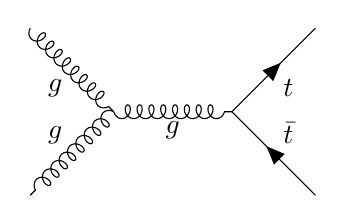
\begin{tikzpicture}
	\begin{feynman}
		\vertex (a);
		\vertex [below right=of a] (b);
		\vertex [below left=of b] (c);
		\vertex [right=of b] (d);
		\vertex [above right=of d] (e);
		\vertex [below right=of d] (f);
		
		\diagram* {
			(a) -- [gluon, edge label'=\(g\)] (b) -- [gluon, edge label'=\(g\)] (c);
			(b) -- [gluon, edge label'=\(g\)] (d);
			(f) -- [fermion, edge label'=\(\bar{t}\)] (d) -- [fermion, edge label'=\(t\)] (e);
		
		};
	\end{feynman}
\end{tikzpicture}

\end{document}
